\begin{center}
	\textbf{CHƯƠNG 8: CHUYỂN ĐỘNG TRÒN}
\end{center}

% ===================================================================
\begin{ex}
	Xét một cung tròn chắn bởi góc ở tâm bằng \SI{1.8}{\radian}. Bán kính đường tròn này bằng \SI{2.4}{\centi\meter}. Chiều dài của cung tròn này và diện tích của hình quạt giới hạn bởi cung tròn có độ lớn lần lượt bằng
	\choice
	{\SI{2.16}{\centi\meter} và \SI{5.18}{\centi\meter^2}}
	{\SI{4.32}{\centi\meter} và \SI{10.4}{\centi\meter^2}}
	{\SI{2.32}{\centi\meter} và \SI{5.18}{\centi\meter^2}}
	{\True\SI{4.32}{\centi\meter} và \SI{5.18}{\centi\meter^2}}
	\loigiai{}
\end{ex}
% ===================================================================
\begin{ex}
	\immini{Một chất điểm M thực hiện chuyển động tròn đều như hình bên dưới.\\
		Nhận xét nào sau đây là đúng?
		\choice
		{$\vec{A}$ là vector vận tốc, $\vec{B}$ là vector gia tốc}
		{$\vec{B}$ là vector vận tốc, $\vec{A}$ là vector gia tốc}
		{\True $\vec{B}$ là vector vận tốc, $\vec{D}$ là vector gia tốc}
		{$\vec{C}$ là vector vận tốc, $\vec{D}$ là vector gia tốc}}
	{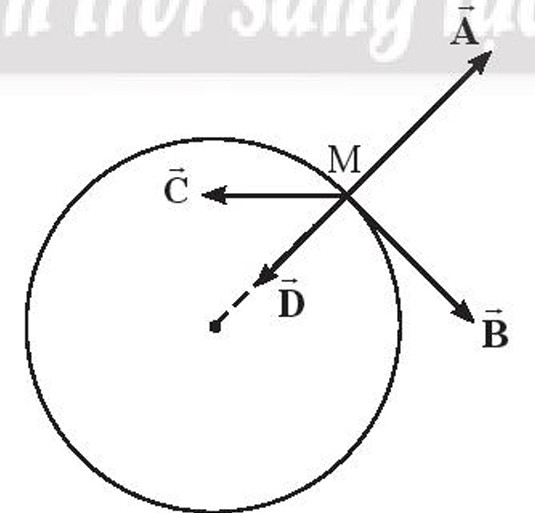
\includegraphics[scale=0.4]{figs/D10-CK2-001-1}}
	\loigiai{}
\end{ex}
% ===================================================================
\begin{ex}
	Chuyển động nào sau đây có thể xem như là chuyển động tròn đều?
	\choice
	{Chuyển động của một vật được ném xiên từ mặt đất}
	{Chuyển động trong mặt phẳng thẳng đứng của một vật được buộc vào một dây có chiều dài cố định}
	{\True Chuyển động của một vệ tinh nhân tạo có vị trí tương đối không đổi đối với một điểm trên mặt đất (vệ tinh địa tĩnh)}
	{Chuyển động của một quả táo khi rời ra khỏi cành cây}
	\loigiai{}
\end{ex}
% ===================================================================
\begin{ex}
	Chuyển động của vật nào dưới đây được coi là chuyển động tròn đều?
	\choice
	{Chuyền động quay của bánh xe ô tô khi đang hãm phanh}
	{Chuyển động của một quả bóng đang lăn đều trên mặt sân}
	{\True Chuyển động quay của điểm treo các ghế ngồi trên chiếc đu quay đang quay đều}
	{Chuyển động quay của cánh quạt khi vừa tắt điện}
	\loigiai{}
\end{ex}
% ===================================================================
\begin{ex}
	Chuyển động tròn đều có
	\choice
	{vector vận tốc không đổi}
	{\True tốc độ phụ thuộc vào bán kính quỹ đạo}
	{tốc độ góc phụ thuộc vào bán kính quỹ đạo}
	{gia tốc hướng tâm tỉ lệ với thời gian chuyển động}
	\loigiai{}
\end{ex}
% ===================================================================
\begin{ex}
	Trên mặt một chiếc đồng hồ treo tường, kim giờ dài \SI{10}{\centi\meter}, kim phút dài \SI{15}{\centi\meter}. Tốc độ góc của kim giờ và kim phút là
	\choice
	{$\SI{1.52E-4}{\radian/\second}$, $\SI{1.82E-3}{\radian/\second}$}
	{\True $\SI{1.45E-4}{\radian/\second}$, $\SI{1.74E-3}{\radian/\second}$}
	{$\SI{1.54E-4}{\radian/\second}$, $\SI{1.91E-3}{\radian/\second}$}
	{$\SI{1.48E-4}{\radian/\second}$, $\SI{1.78E-3}{\radian/\second}$}
	\loigiai{}
\end{ex}
% ===================================================================
\begin{ex}
	Một hòn đá buộc vào sợi dây có chiều dài \SI{1}{\meter}, quay đều trong mặt phẳng thẳng đứng với tốc độ 60 vòng/phút. Thời gian để hòn đá quay hết một vòng và tốc độ của nó là
	\choice
	{\True \SI{1}{\second}; \SI{6.28}{\meter/\second}}
	{\SI{1}{\second}; \SI{2}{\meter/\second}}
	{\SI{3.14}{\second}; \SI{1}{\meter/\second}}
	{\SI{6.28}{\second}; \SI{3.14}{\meter/\second}}
	\loigiai{}
\end{ex}
% ===================================================================
\begin{ex}
	Một vệ tinh nhân tạo chuyển động tròn đều quanh Trái Đất ở độ cao bằng bán kính $R$ của Trái Đất. Lấy gia tốc rơi tự do tại mặt đất là $g=\SI{10}{\meter/\second^2}$ và bán kính của Trái Đất bằng $R=\SI{6400}{\kilo\meter}$. Thời gian vệ tinh quay quanh Trái Đất hết 1 vòng là
	\choice
	{2 giờ 48 phút}
	{\True 1 giờ 59 phút}
	{3 giờ 57 phút}
	{1 giờ 24 phút}
	\loigiai{}
\end{ex}
% ===================================================================
\begin{ex}
	Câu nào sau đây nói về gia tốc trong chuyển động tròn đều là \textbf{sai}?
	\choice
	{Vector gia tốc luôn hướng vào tâm quỹ đạo}
	{Độ lớn của gia tốc $a=\dfrac{v^2}{R}$, với $v$ là tốc độ, $R$ là bán kính quỹ đạo}
	{\True Gia tốc đặc trưng cho sự biến thiên về độ lớn của vận tốc}
	{Vector gia tốc luôn vuông góc với vector vận tốc ở mọi thời điểm}
	\loigiai{}
\end{ex}
% ===================================================================
\begin{ex}
	Phát biểu nào sau đây là đúng?\\
	Trong chuyển động tròn đều
	\choice
	{vector vận tốc luôn không đổi, do đó gia tốc bằng 0}
	{gia tốc hướng vào tâm quỹ đạo, độ lớn tỉ lệ nghịch với bình phương tốc độ}
	{phương, chiều và độ lớn của vận tốc luôn thay đổi}
	{\True gia tốc hướng vào tâm quỹ đạo, độ lớn tỉ lệ với bình phương tốc độ góc}
	\loigiai{}
\end{ex}
% ===================================================================
\begin{ex}
	Một vệ tinh nhân tạo chuyển động tròn đều quanh Trái Đất, mỗi vòng hết 90 phút. Vệ tinh bay ở độ cao \SI{320}{\kilo\meter} so với mặt đất. Biết bán của kính Trái Đất là \SI{6380}{\kilo\meter}. Tốc độ và gia tốc hướng tâm của vệ tinh là
	\choice
	{\True \SI{7792}{\meter/\second}; \SI{9.062}{\meter/\second^2}}
	{\SI{7651}{\meter/\second}; \SI{8.120}{\meter/\second^2}}
	{\SI{6800}{\meter/\second}; \SI{7.892}{\meter/\second^2}}
	{\SI{7902}{\meter/\second}; \SI{8.960}{\meter/\second^2}}
	\loigiai{}
\end{ex}
% ===================================================================
\begin{ex}
	Chọn đáp án đúng khi nói về vector gia tốc của vật chuyển động tròn đều.
	\choice
	{Có độ lớn bằng 0}
	{Giống nhau tại mọi điểm trên quỹ đạo}
	{Luôn cùng hướng với vector vận tốc}
	{\True Luôn vuông góc với vector vận tốc}
	\loigiai{}
\end{ex}
% ===================================================================
\begin{ex}
	\SI{1}{\radian} là số đo góc ở tâm một đường tròn chắn cung có độ dài bằng
	\choice
	{\True bán kính đường tròn đó}
	{đường kính đường tròn đó}
	{nửa chu vi đường tròn đó}
	{chu vi đường tròn đó}
	\loigiai{}
\end{ex}

% ===================================================================
\begin{ex}
	Một vật chuyển động tròn đều với quỹ đạo có bán kính $r$, tốc độ góc $\omega$. Biểu thức liên hệ giữa gia tốc hướng tâm $a$ của vật với tốc độ góc $\omega$ và bán kính $r$ là
	\choice
	{$a=\omega r$}
	{$\sqrt{\omega}=\dfrac{a}{r}$}
	{\True $\omega=\sqrt{\dfrac{a}{r}}$}
	{$a=\omega r^2$}
	\loigiai{}
\end{ex}




\Closesolutionfile{ans}
\newpage
\begin{center}
	\textbf{ĐÁP ÁN}
\end{center}
\inputansbox{10}{ans/ONTAPHK2-TN}
